\newpage
\section{Amplificadores realimentados por corriente (CFA)}
\subsection{Introducción}
Este tipo de amplificador pertenece al grupo de aquellos que para operar linealmente, deben ser realimentados negativamente debido a su elevada ganancia de lazo abierto. No obstante presentan características funcionales dinámicas distintas al operacional clásico (VFA). La diferencia de arquitectura, principalmente de la etapa de entrada y además el menor número de estas, resultan en aumento de velocidad, tanto en pequeña como en gran señal, con rangos de operación superiores a $100\,\text{MHz}$ y más de $1000\,\text{V}/\mu\text{s}$ respectivamente, mostrando producto ganancia ancho de banda del orden del GHz, aunque la precisión en continua es en general más pobre que aquellos.

La figura \ref{fig:3.1} muestra un modelo compacto del amplificador realimentado por corriente también denominado de Transimpedancia, nombre justificado por el hecho que, el generador de tensión de salida está controlado por la corriente de señal de la entrada inversora ($I_{\text{in}}$), terminal este, de muy baja impedancia (ej. $20\,\Omega$), que se corresponde con el de salida del buffer cuya entrada, de muy alta impedancia, configura la no inversora.
\begin{figure}[H]
    \centering
    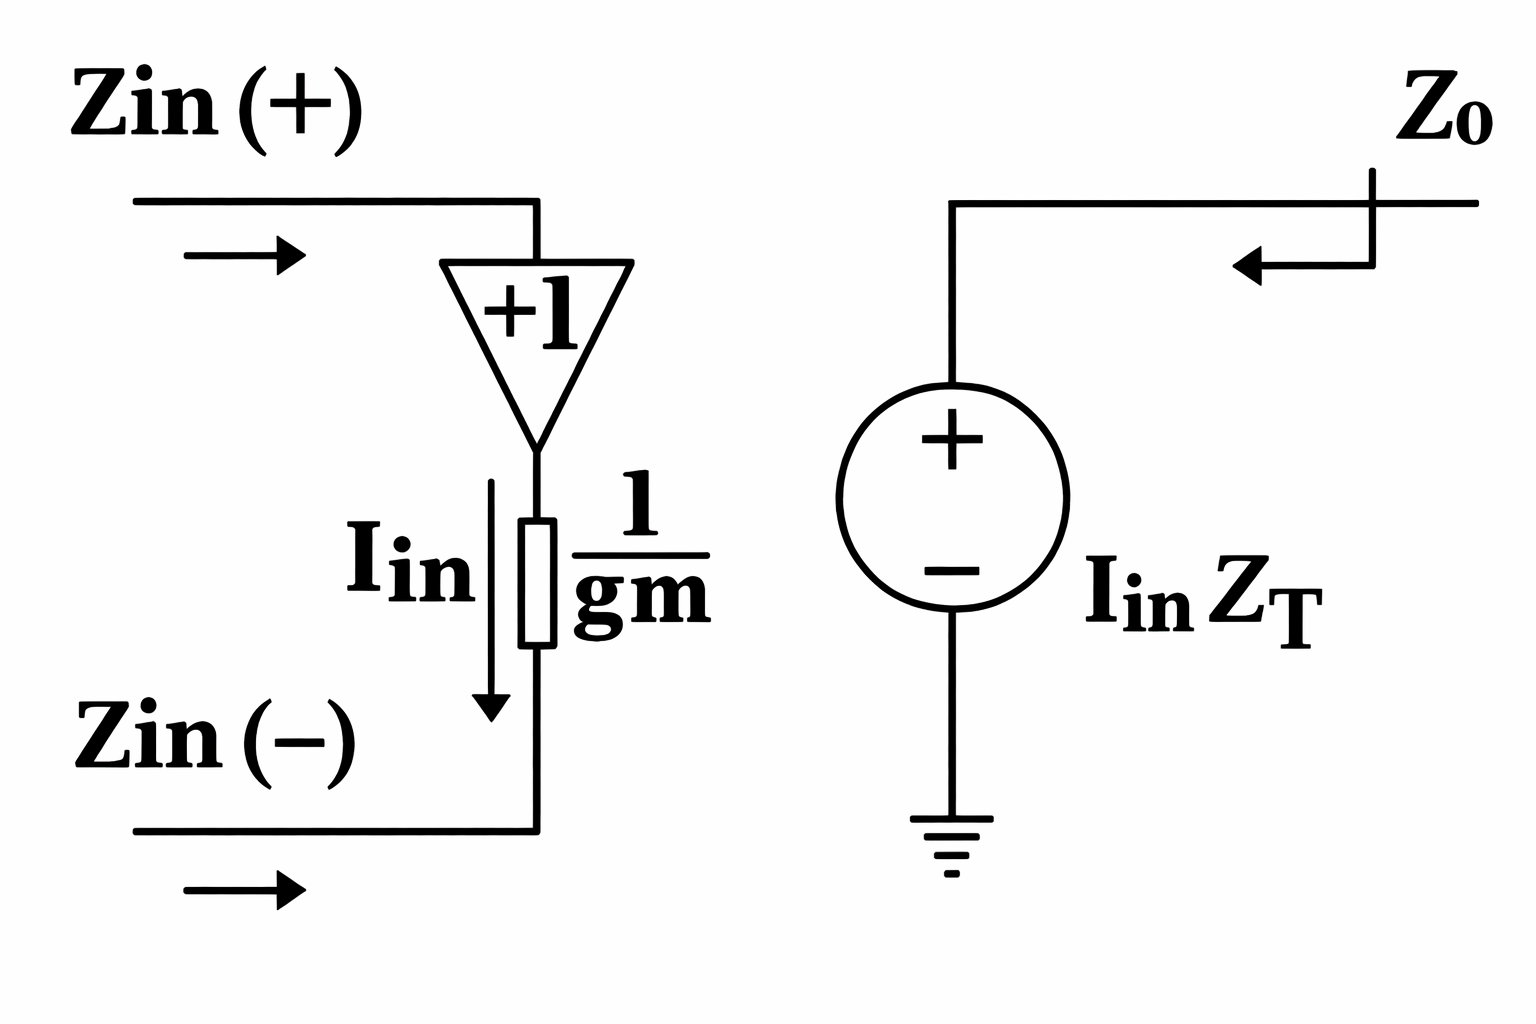
\includegraphics[width=0.5\linewidth]{Imagenes/3.1.png}
    \caption{CFA}
    \label{fig:3.1}
\end{figure}
La transimpedancia $Z_T(s)$, puede ser aproximada en la banda de utilización por una función de transferencia de un solo polo como lo indica (\ref{eq:3.1})

\begin{equation}
Z_t(s) = \frac{R_t}{1 + s R_t C_t}
\label{eq:3.1}
\end{equation}

Donde, $R_t$ y $C_t$ se denominan transresistencia y transcapacitancia respectivamente, con valores típicos en torno al megaohm y los $2\,\text{pF}$ respectivamente. La transimpedancia es publicada en hojas de dato, en diagramas de módulo y fase, mostrando esta última polos de segundo orden cuyo, efecto sobre la respuesta será analizado posteriormente en temas relativos a la estabilidad del amplificador. A continuación se analizará la respuesta de las configuraciones típicas.
\subsection{Respuesta en frecuencia}
Se evaluará  la respuesta del amplificador en la configuración no inversora de (\ref{fig:3.2}), idealizando el 
Buffer de entrada
\begin{figure}[H]
    \centering
    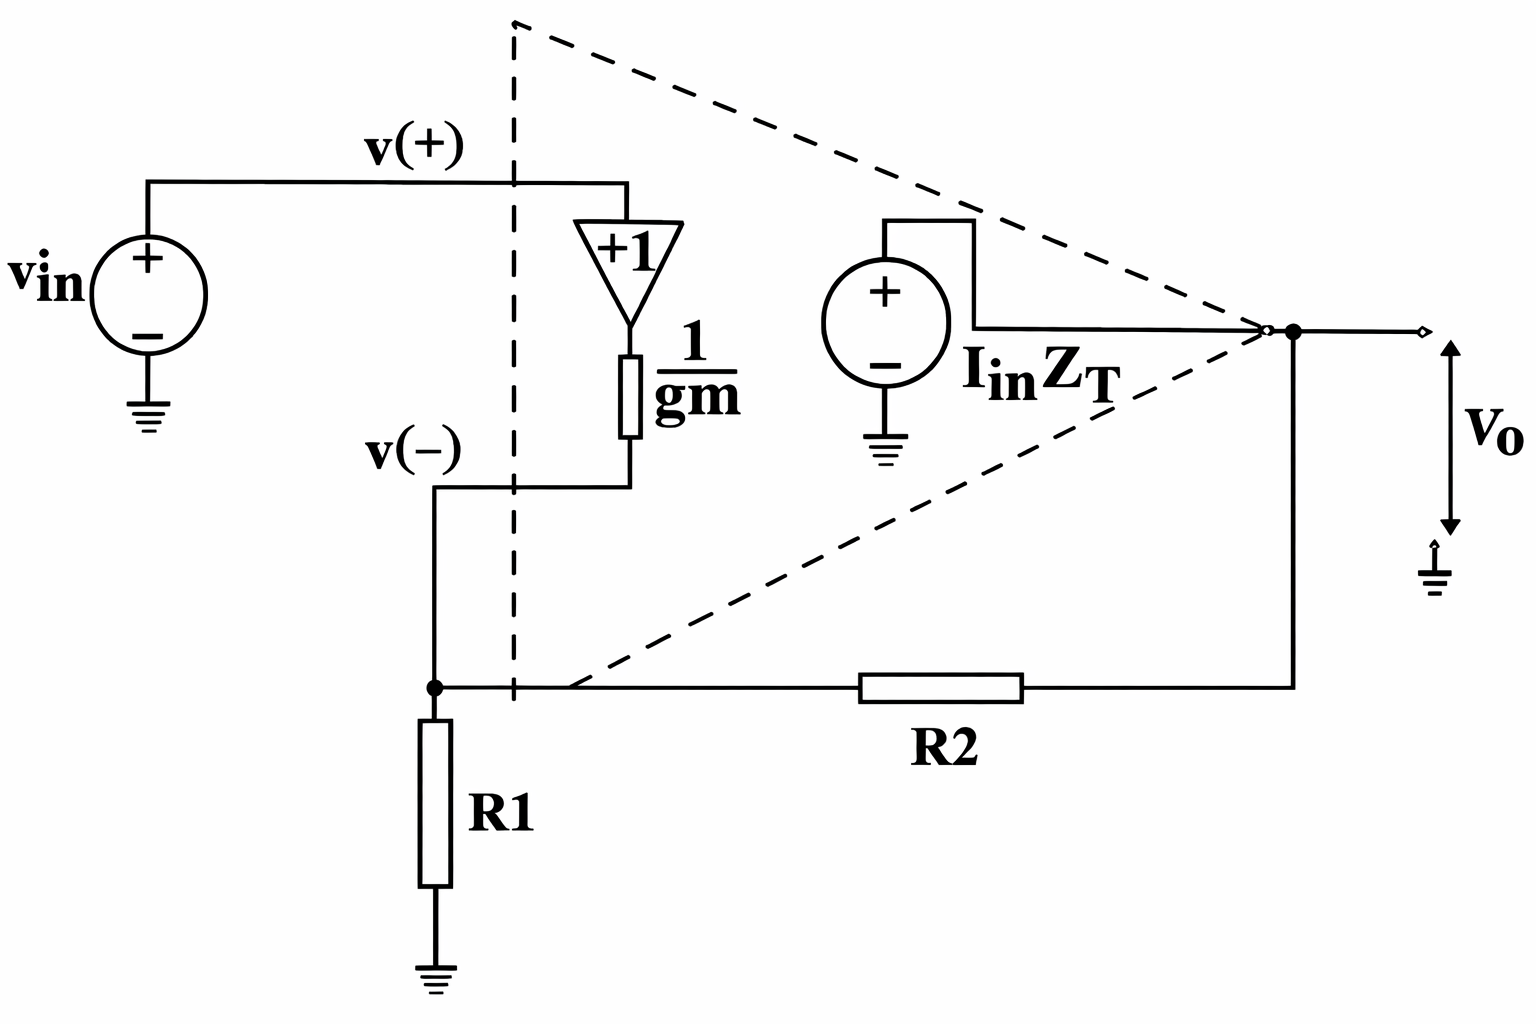
\includegraphics[width=0.5\linewidth]{Imagenes/3.2.png}
    \caption{}
    \label{fig:3.2}
\end{figure}
La apertura del lazo de la (\ref{fig:3.3}) prepara convenientemente al amplificador para efectuar el análisis 
propuesto utilizando la expresión de Black. 
\begin{figure}[H]
    \centering
    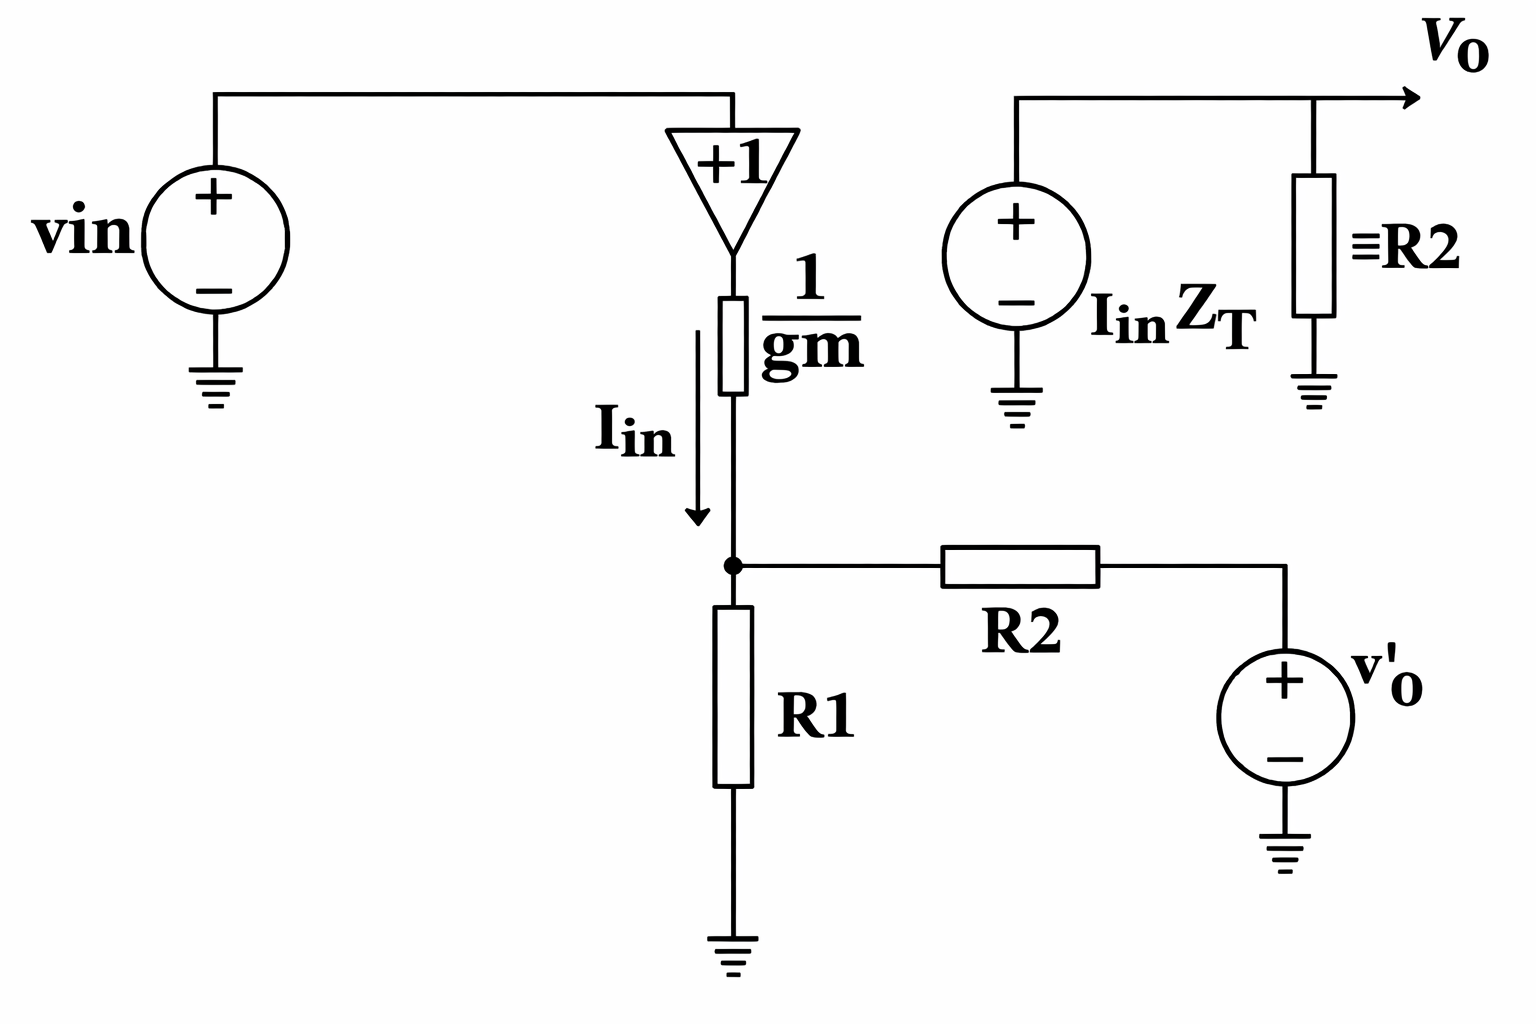
\includegraphics[width=0.5\linewidth]{Imagenes/3.3.png}
    \caption{}
    \label{fig:3.3}
\end{figure}
Considerar ideal el buffer de entrada implica que
$Z_{in+} = \infty$; $Z_{in-} = 0$ y $V_+ = V_-$.

Luego la ganancia de lazo abierto evaluada arroja el siguiente resultado:

\begin{equation}
GLA = \frac{V_o}{V'_{in}} = \frac{I_{in} Z_t}{I_{in} (R_1 \parallel R_2)} = \frac{Z_t}{R_1 \parallel R_2}
\label{eq:3.2}
\end{equation}
De igual manera la ganancia de lazo resulta:

\begin{equation}
GL|_{v'_{in}=0} = \left( \frac{v_0}{v'} \right) = - \frac{Z_t}{R_2}
\label{eq:3.3}
\end{equation}

Finalmente la ganancia de lazo cerrado es

\begin{equation}
A_{vf} = \left( \frac{v_0}{v_{IN}} \right) == \frac{\frac{Z_t}{R_p}}{1 + \frac{Z_t}{R_2}} = \frac{R_2 / R_p}{1 + \frac{1}{Z_t / R_2}} = \frac{\overbrace{1 + R_2 / R_1}^{Avfi}}{1 - \frac{1}{T}}
\label{eq:3.4}
\end{equation}

La expresión final de ecuación anterior, muestra la forma clásica de la ganancia no inversora del amplificador realimentado con función de transferencia de un solo polo, en términos de su valor idealizado, con el término de error producido por la ganancia de lazo finita.

$$
\varepsilon = \frac{1}{T(s)}
$$

La expresión (\ref{eq:3.2}), pone en evidencia el efecto de la baja impedancia de la entrada inversora ya que debido a esto, es inevitable que la red de realimentación cargue a la misma, haciendo que la ganancia de lazo abierto dependa inversamente de $R_p$ de la misma manera que la ganancia de lazo cerrado ($R_2/R_p$).. Esto muestra la diferencia operativa básica que tiene la CFA respecto del operacional clásico donde GLA es prácticamente invariante con la cantidad de realimentación introducida, debido a que ambas entradas son de alta impedancia

Otra diferencia relevante a remarcar, se refiere al comportamiento dinámico del CFA, que se pone en evidencia desarrollando el denominador (\ref{eq:3.4}), según se muestra a continuación

\begin{equation}
1 + \frac{1}{\frac{Z_t}{R2}} = 1 + \frac{R_2}{R_t} + sC_t R_2 \cong 1 + sC_t R_2
\label{eq:3.5}
\end{equation}

En la anterior es $R_2/Rt << 1$, debido a que por razones de optimización del comportamiento dinámico, $R_2$ debe ser del orden de $1 \text{ k}\Omega$.
Finalmente GLC puede expresarse como

\begin{equation}
Avf_{(s)} = \frac{R_2 / R_p}{1 + sC_t R_2} = \frac{Avfi}{1 + s/ \omega_H}
\label{eq:3.6}
\end{equation}

\begin{equation}
\omega_H = 1/CtR2
\label{eq:3.7}
\end{equation}

El análisis realizado permite extraer conclusiones relevantes respecto del comportamiento dinámico del CFA. Por ejemplo, si se varia la ganancia de señal $R_2/R_p=1+R_2/R_1$ , a través de $R_1$ y manteniendo constante $R_2$, tanto el ancho de banda como la ganancia del lazo, $T(s)$, permanecen constantes, mientras que la ganancia de lazo abierto varia en el mismo sentido y magnitud que la de señal. Una consecuencia de esto es que tenga característica producto Ganancia- Ancho de Banda, creciente con la ganancia pudiendo llegar al GHz.
La (\ref{fig:3.4}) muestra en diagrama de Bode, las magnitudes de las ecuaciones desarrolladas, dando una 
clara visión del comportamiento del dispositivo para dos diferentes ganancias de lazo cerrado. 
\begin{figure}[H]
    \centering
    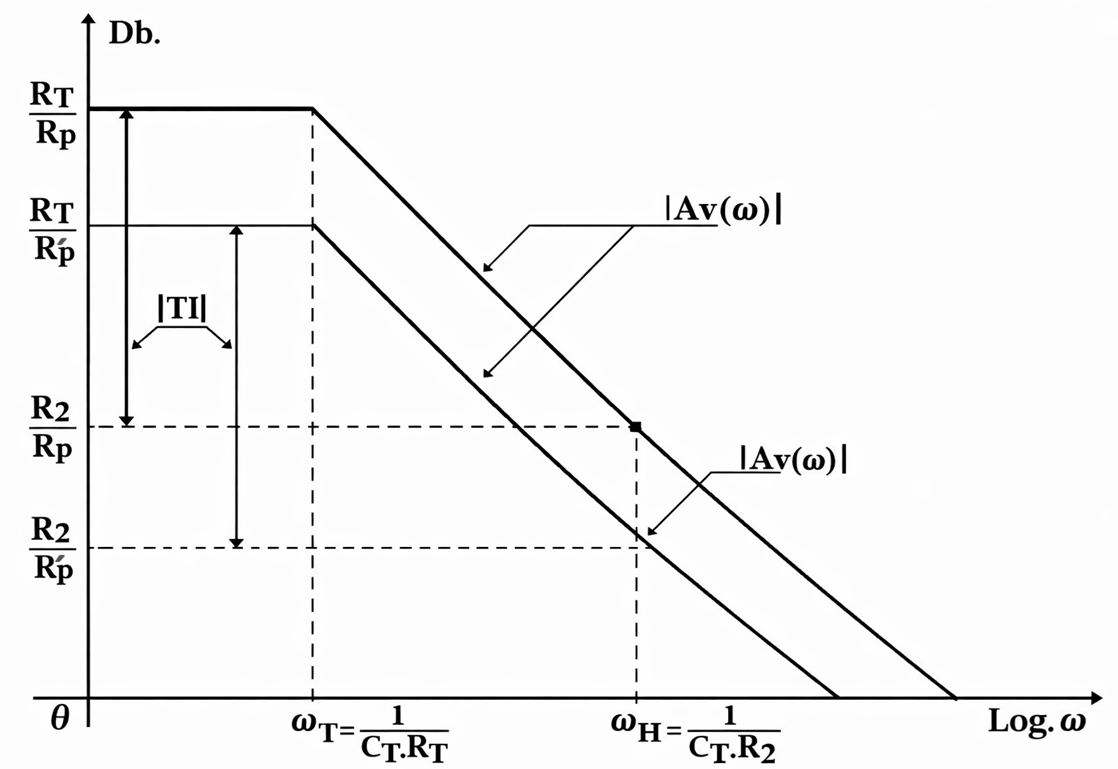
\includegraphics[width=0.5\linewidth]{Imagenes/3.4.png}
    \caption{}
    \label{fig:3.4}
\end{figure}
Las conclusiones obtenidas se pueden extender a otras configuraciones amplificadoras, así por ejemplo la respuesta de una configuración inversora se deduce de fig \ref{fig:3.3}, excitando con el generador de señal el extremo de R1, del que se obtienen las siguientes relaciones.

\begin{equation}
GLA|_{V'=0} = \left( \frac{v_0}{I_{in}} \right) \left( \frac{I_{IN}}{V_{in}} \right) = Z_t . \left( - \frac{1}{R_1} \right) = - \frac{Z_t}{R_1}
\label{eq:3.8}
\end{equation}

La ganancia de lazo, independiente del punto de inyección de señal, responde a la expresión deducida en (\ref{eq:3.3}).

Finalmente se obtiene para la ganancia de lazo cerrado la siguiente ecuación

\begin{equation}
A_{vf} = \left( \frac{v_0}{V_{in}} \right) = \frac{- \frac{Z_t}{R_1}}{1 + \frac{Z_t}{R_2}} = \frac{- R_2 / R_1}{1 + \frac{1}{Z_t / R_2}} = \frac{\overbrace{- R_2 / R_1}^{Avfi}}{1 - \frac{1}{T}}
\label{eq:3.9}
\end{equation}

Utilizando el desarrollo del denominador de la expresión dada en (\ref{eq:3.6}), la anterior se expresa:

El procedimiento de diseño del amplificador comienza con la selección de la resistencia de realimentación ($R_2$), para fijar el ancho de banda y cuyo valor tiene un mínimo dado por razones de estabilidad, tema que será analizado en detalle en secciones posteriores. No obstante en la hoja de datos del dispositivo se recomienda un valor, (En torno al $\text{k}\Omega$), que optimiza en términos de estabilidad su operación dinámica. Debido a esto para implementar un amplificador separador (Buffer), a diferencia del caso VFA, se debe hacer, $R_1= \infty$ y $R_2 \neq 0$, por las razones arriba comentadas.
La resistencia $R_1$, es fijada por requerimiento de ganancia de lazo cerrado, obviamente el incremento de esta implica disminución de la primera de modo que para ganancias elevadas el valor de $R_1$ es comparable con la impedancia de entrada no inversora ($R_{IN} = 1/gm \approx 30 \text{ Ohms}$) que fue supuesta nula en el análisis precedente pero dejaría de serlo en la situación planteada. Las expresiones encontradas en las configuraciones analizadas se pueden modificar teniendo en cuenta este efecto. Por ejemplo para la no inversora se obtiene de figura 3.3

\begin{equation}
GLA|_{v'=0} = \left( \frac{v_0}{v_{in}} \right) = \frac{Z_t}{R_{IN} + R_p}
\label{eq:3.10}
\end{equation}

La anterior se puede expresar de manera diferente multiplicado y dividiendo por la ganancia de lazo cerrado no inversora ideal ($(Avfi)_N$) y desarrollando el denominador resultante.

$$
GLA|_{v'=0} = \left( \frac{v_0}{v_{IN}} \right) = \frac{Z_t \overbrace{(1 + R_2 / R_1)}^{(Avfi)_{NI}}}{(R_{IN} + R_p)(1 + R_2 / R_1)} = \frac{Z_t (A_{vfi})_{NI}}{R_2 + R_{IN} (A_{vfi})_{NI}}
$$

La ganancia de lazo ($T$) resulta

\begin{equation}
GL|_{vin'=0} = \left( \frac{v_0}{v'} \right) = - \left( \frac{Z_t}{R_2 + (R_{IN} // R_1)} \right) \left( \frac{R_1}{R_{IN} + R_1} \right) = - \frac{Z_t}{R_2 + R_{IN} (A_{vfi})_{NI}}
\label{eq:3.11}
\end{equation}

Finalmente la ganancia de lazo cerrado es

\begin{equation}
GLC = \left( \frac{v_0}{v_{IN}} \right) = \frac{(A_{vfi})_{NI}}{1 + \frac{R_2 + R_{IN}(A_{vfi})_{NI}}{Z_t}} = \frac{(A_{vfi})_{NI}}{1 - \frac{1}{T}}
\label{eq:3.12}
\end{equation}

Repitiendo el análisis para la configuración inversora de obtiene

$$
GLA|_{V'=0} = \left( \frac{v_0}{v_{in}} \right) = - \frac{Z_t}{(R_1 + (R_{IN} // R_1)).(\frac{R_{IN} + R_2}{R_2})}
$$

La anterior luego de un tratamiento algebraico semejante al realizado en (3.11) se expresa según la siguiente.

\begin{equation}
GLA|_{V'=0} = \left( \frac{v_0}{v_{in}} \right) = \frac{Z_t (A_{vfi})_{In}}{R_2 + R_{IN} (A_{vfi})_{NI}}
\label{eq:3.13}
\end{equation}

Relacionando la anterior con la ganancia de lazo (3.11), se obtiene

\begin{equation}
GLC = \left( \frac{v_0}{v_{in}} \right) = \frac{(A_{vfi})_{In}}{1 + (\frac{R_2 + R_{IN}(A_{vfi})_{NI}}{Z_t})} = \frac{(A_{vfi})_I}{1 - \frac{1}{T}}
\label{eq:3.14}
\end{equation}
\subsection{Errores}
En general este amplificador tiene especificaciones de fuentes de errores en continua más pobres que el VFA y no obstante el análisis de sus efectos es similar al caso anterior, el tratamiento referente a las corrientes de polarización es diferente debido a la asimetría estructural de las entradas no inversora e inversora. Por esto es que la técnica de ecualización de las impedancias vistas desde ambas entradas utilizadas para minimizar el error de corrientes de polarización en el A.O, no sea aplicable al CFA, tal es así que no se publica el offset de corriente, ($I_{OS}$). Es aconsejable analizar las especificaciones de la hoja de datos antes de tomar alguna medida correctiva.

El offset de tensión es elevado, (Ej. $5\text{mV}$) y es generalmente el error que domina en baja frecuencia

\begin{equation}
\Delta v_0 = \pm V_{os} . (A_{vfi})_{NI}
\label{eq:3.17}
\end{equation}

La evaluación de los errores producidos por la ganancia de lazo abierto no ideal, (transimpedancia finita), tiene un tratamiento similar al caso VFA, ya que tanto el de continua como los dinámicos se derivan de la misma expresión general, (Ej. Ecuación. 3.4 y 3.14).